In this section, we present the final results for each individual verilog filed we have submitted:

\subsection{Multi stage path for delay measurements}
The multi stage path was submitted with no issues ans the
\begin{figure}[H]
    \centering
    \begin{subfigure}[b]{0.45\textwidth}
        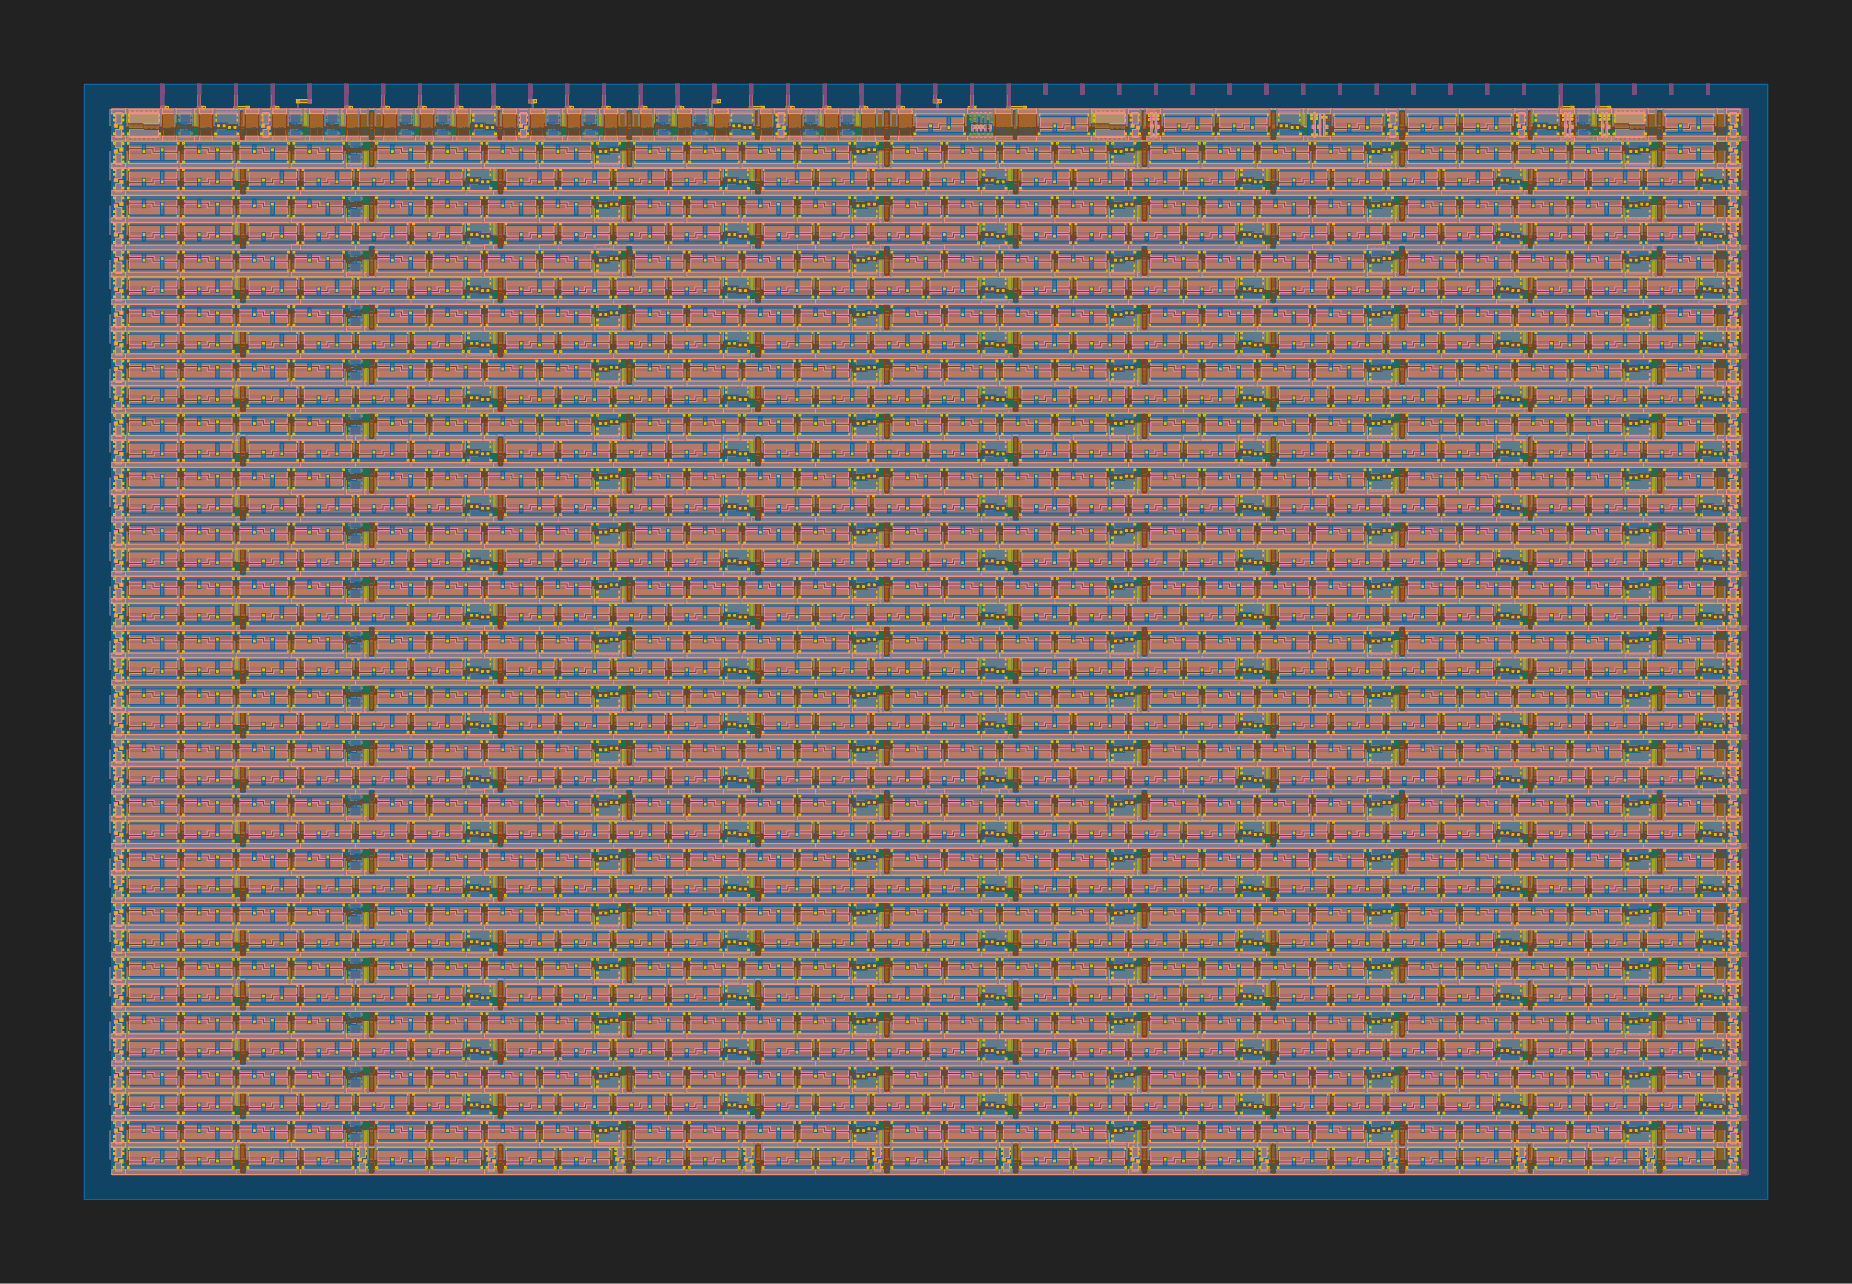
\includegraphics[width=\linewidth]{Pictures/Result_Delay_2D_View.png}
        \caption{View 2D}\label{fig:PWM_2D}
    \end{subfigure}
    \begin{subfigure}[b]{0.45\textwidth}
        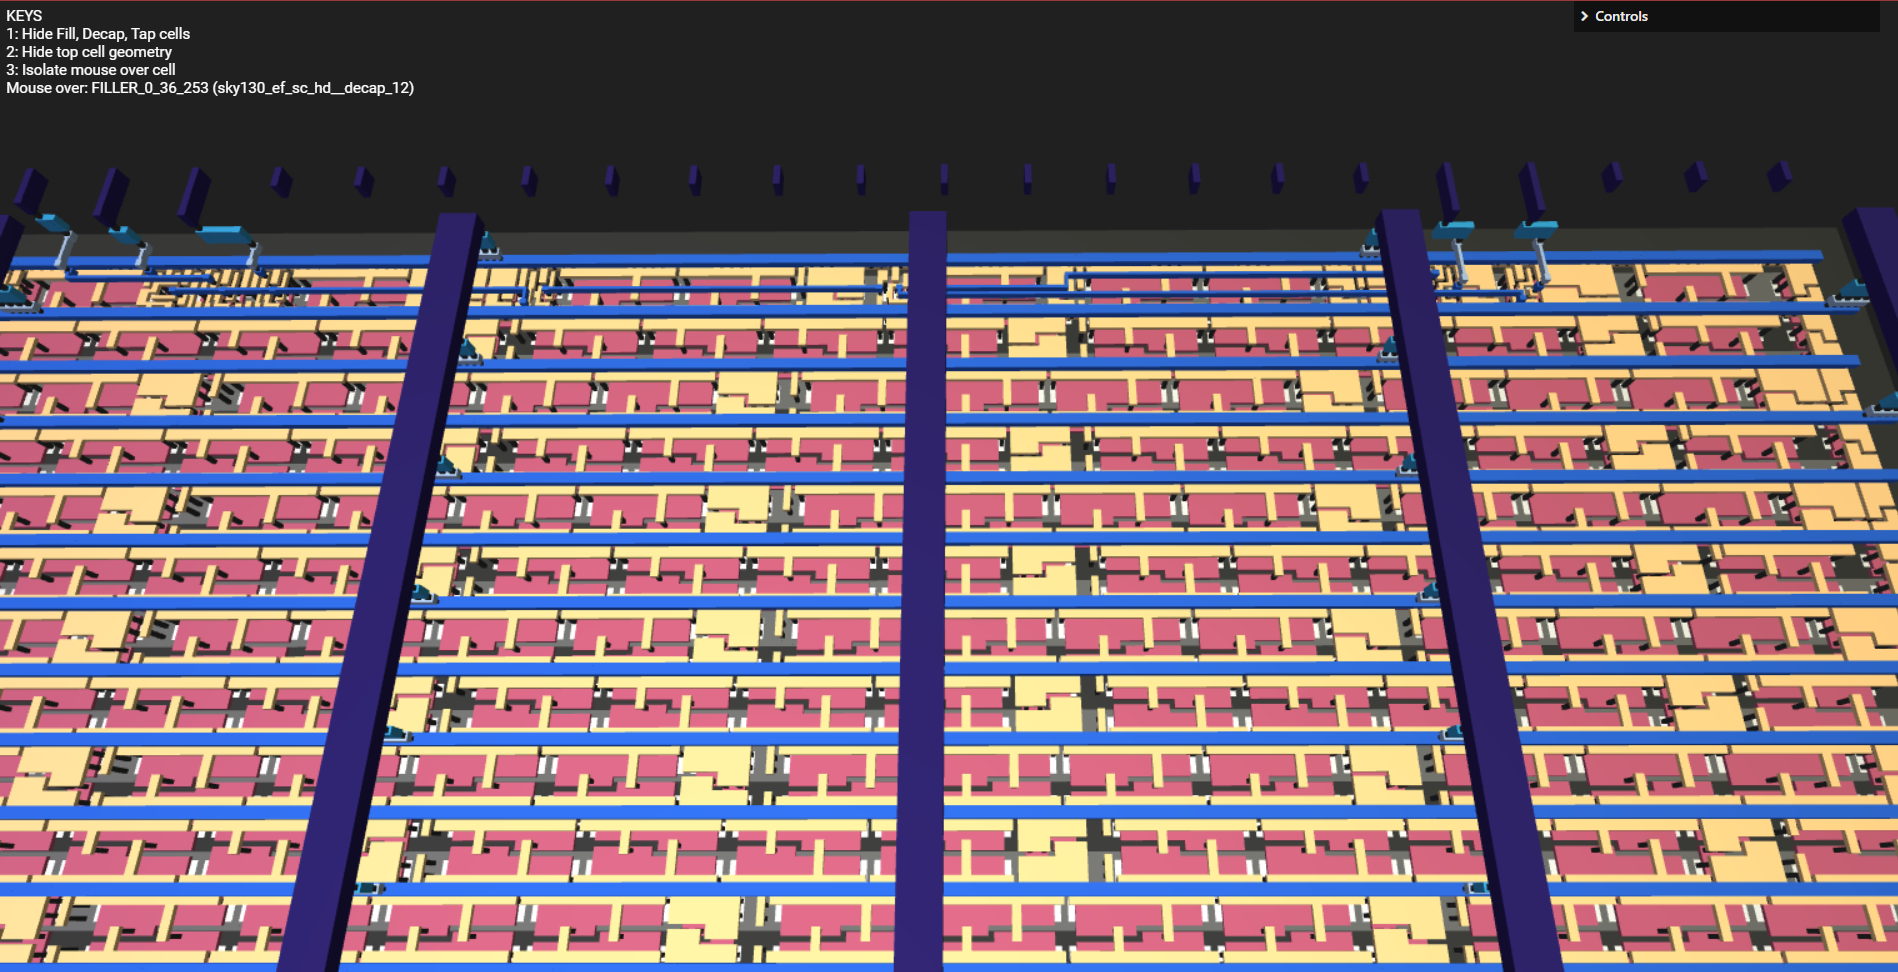
\includegraphics[width=\linewidth]{Pictures/Result_Delay_3D_View.png}
        \caption{View 3D}\label{fig:PWM_3D}
    \end{subfigure}
    \caption{Multi stage path for delay measurements layout}\label{fig:PWM}
\end{figure}



\subsection{ASCII Text Printer Circuit}
Here we've used close to 
\begin{figure}[H]
    \centering
    \begin{subfigure}[b]{0.45\textwidth}
        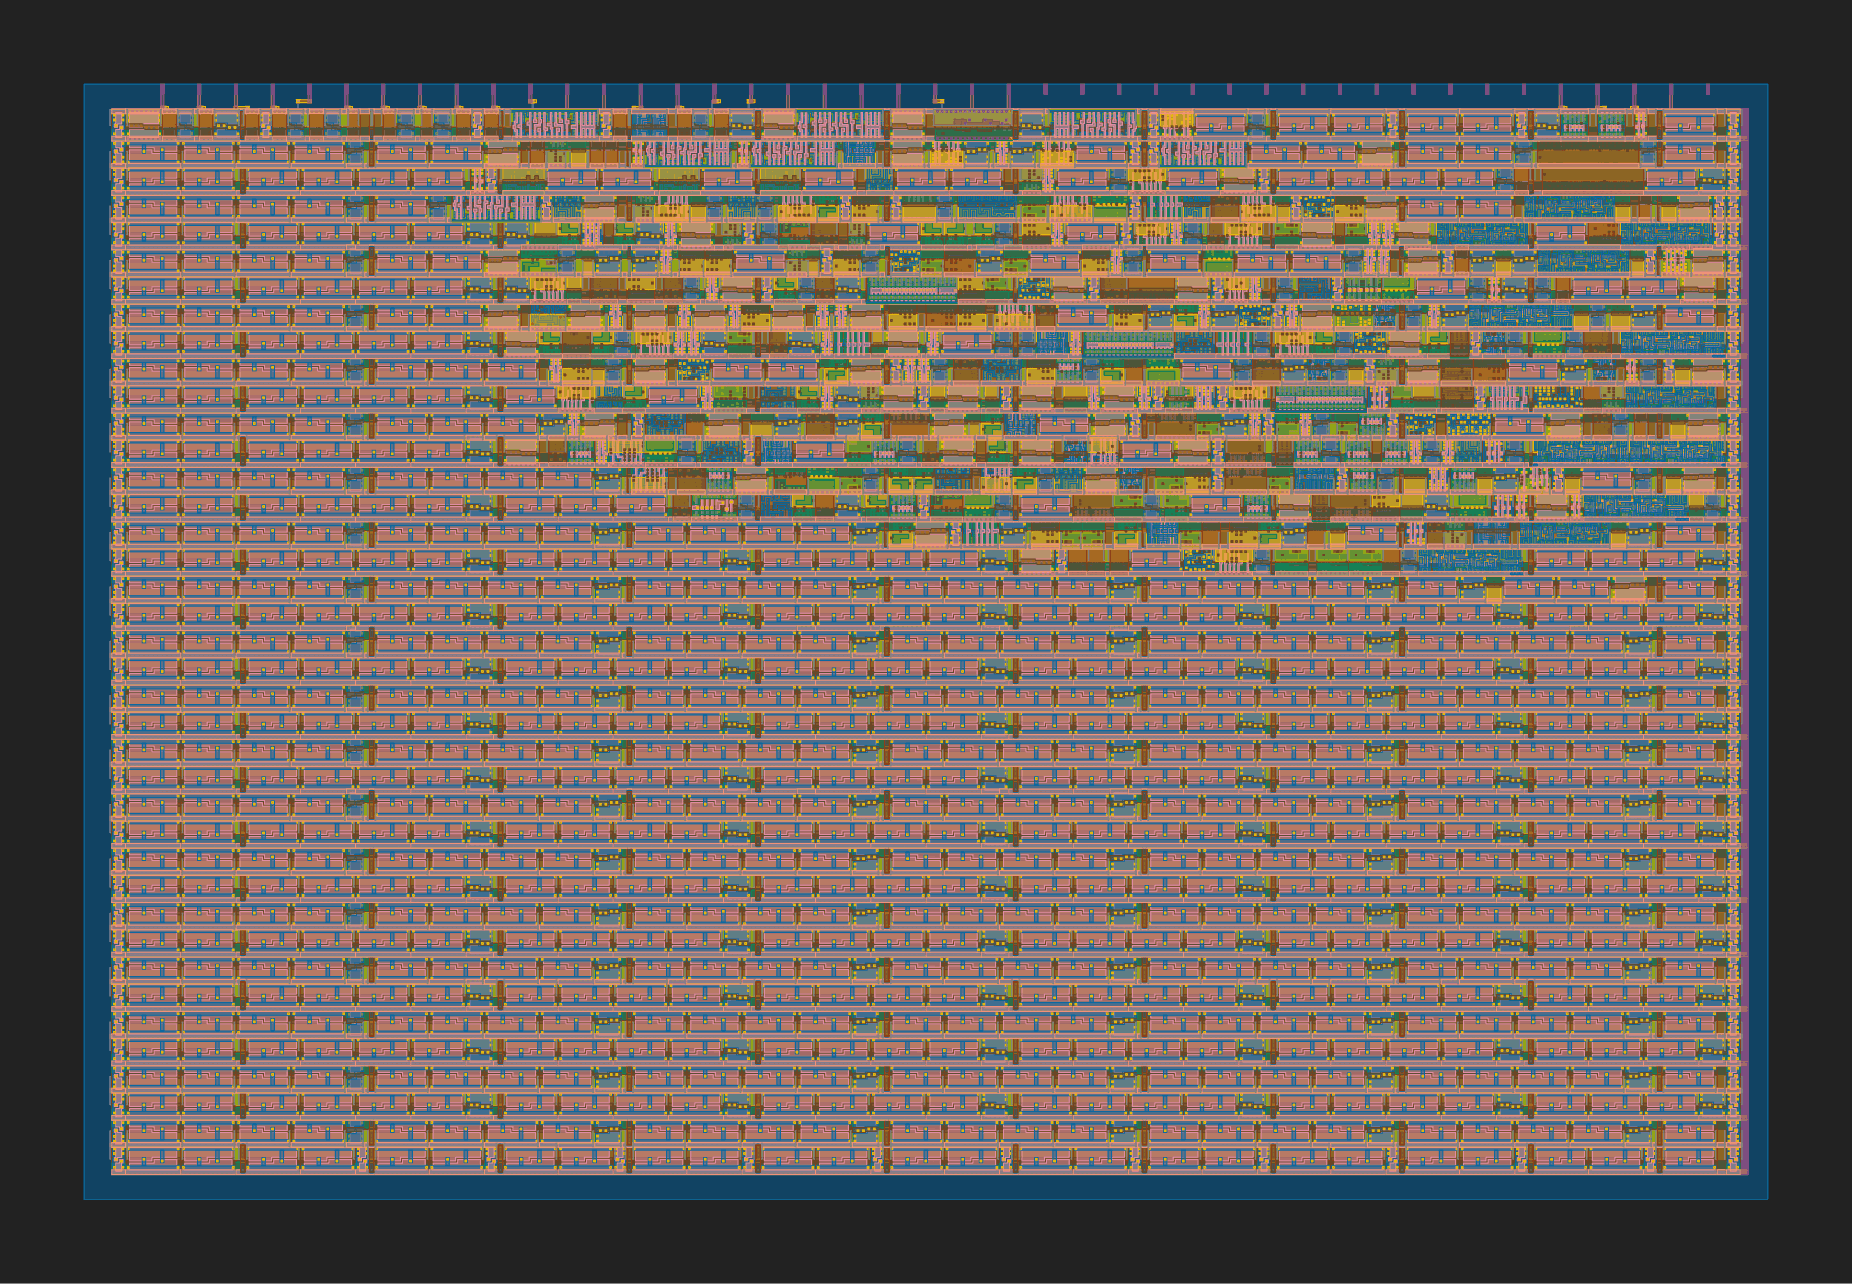
\includegraphics[width=\linewidth]{Pictures/Result_ASCII_2D_View.png}
        \caption{View 2D}\label{fig:PWM_2D}
    \end{subfigure}
    \begin{subfigure}[b]{0.45\textwidth}
        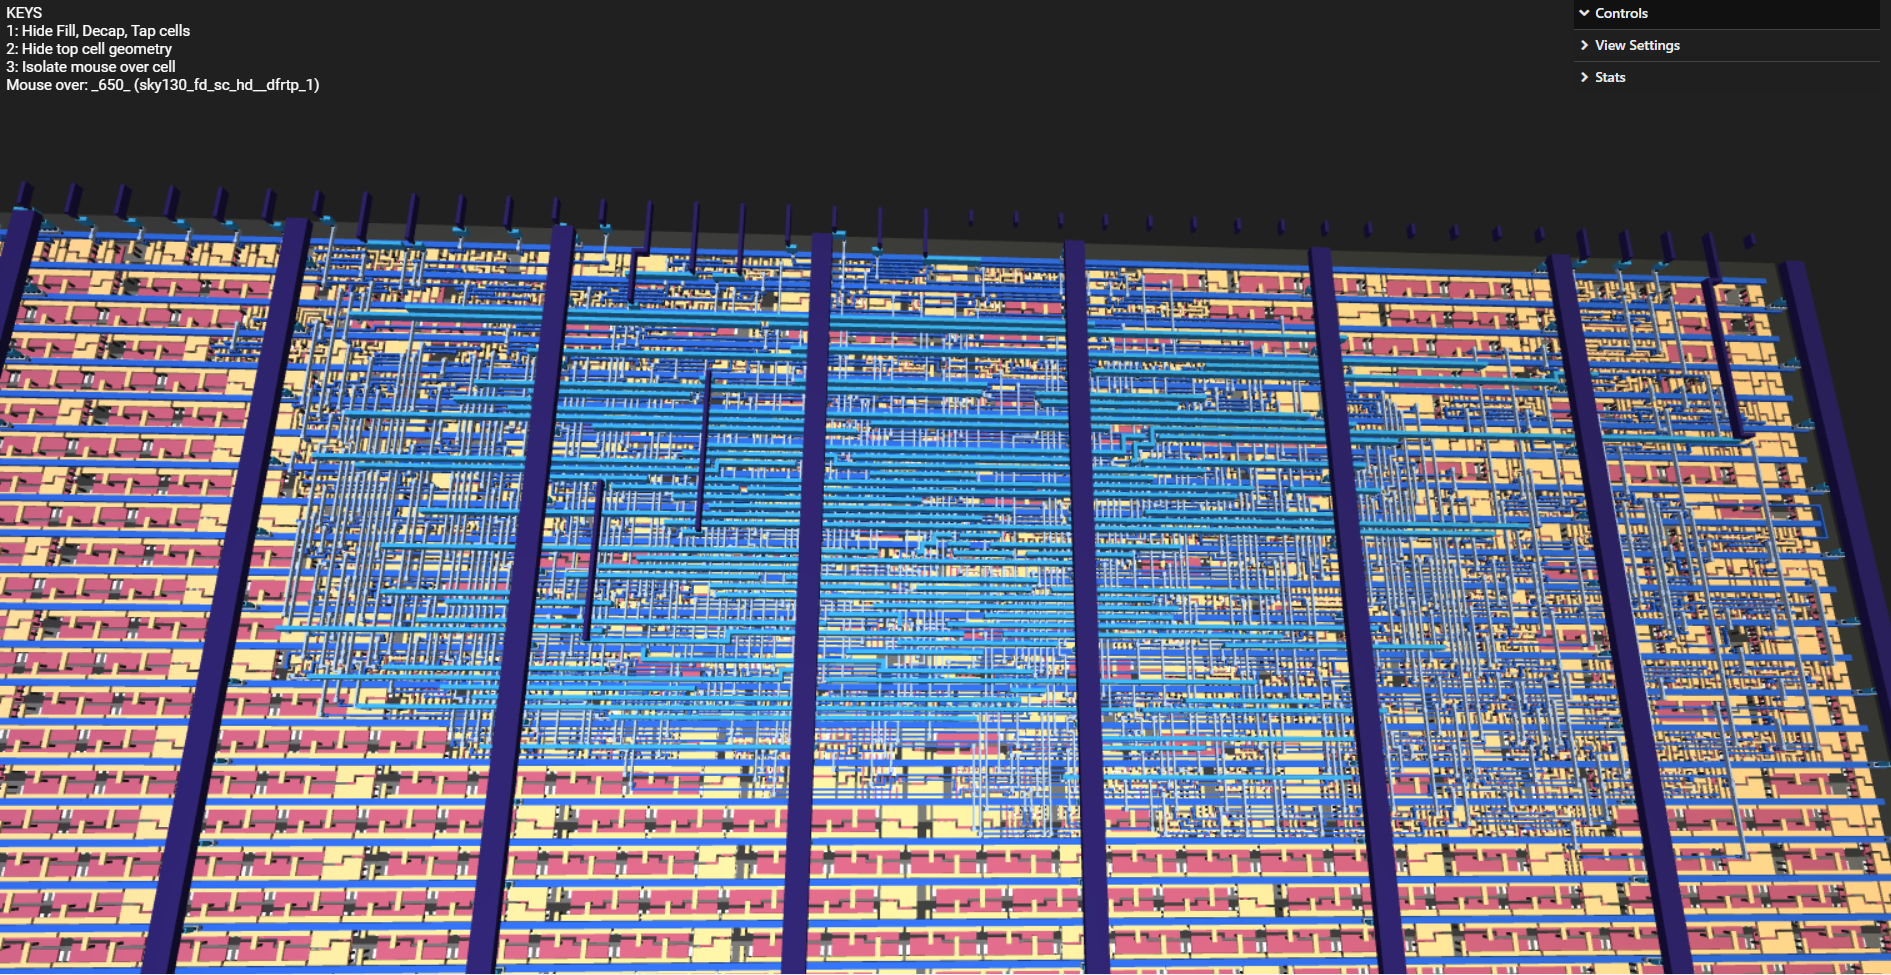
\includegraphics[width=\linewidth]{Pictures/Result_ASCII_3D_View.png}
        \caption{View 3D}\label{fig:PWM_3D}
    \end{subfigure}
    \caption{ASCII text printer circuit layout}\label{fig:PWM}
\end{figure}

\subsection{Implementation of the Pong game}

\begin{figure}[H]
    \centering
    \begin{subfigure}[b]{0.45\textwidth}
        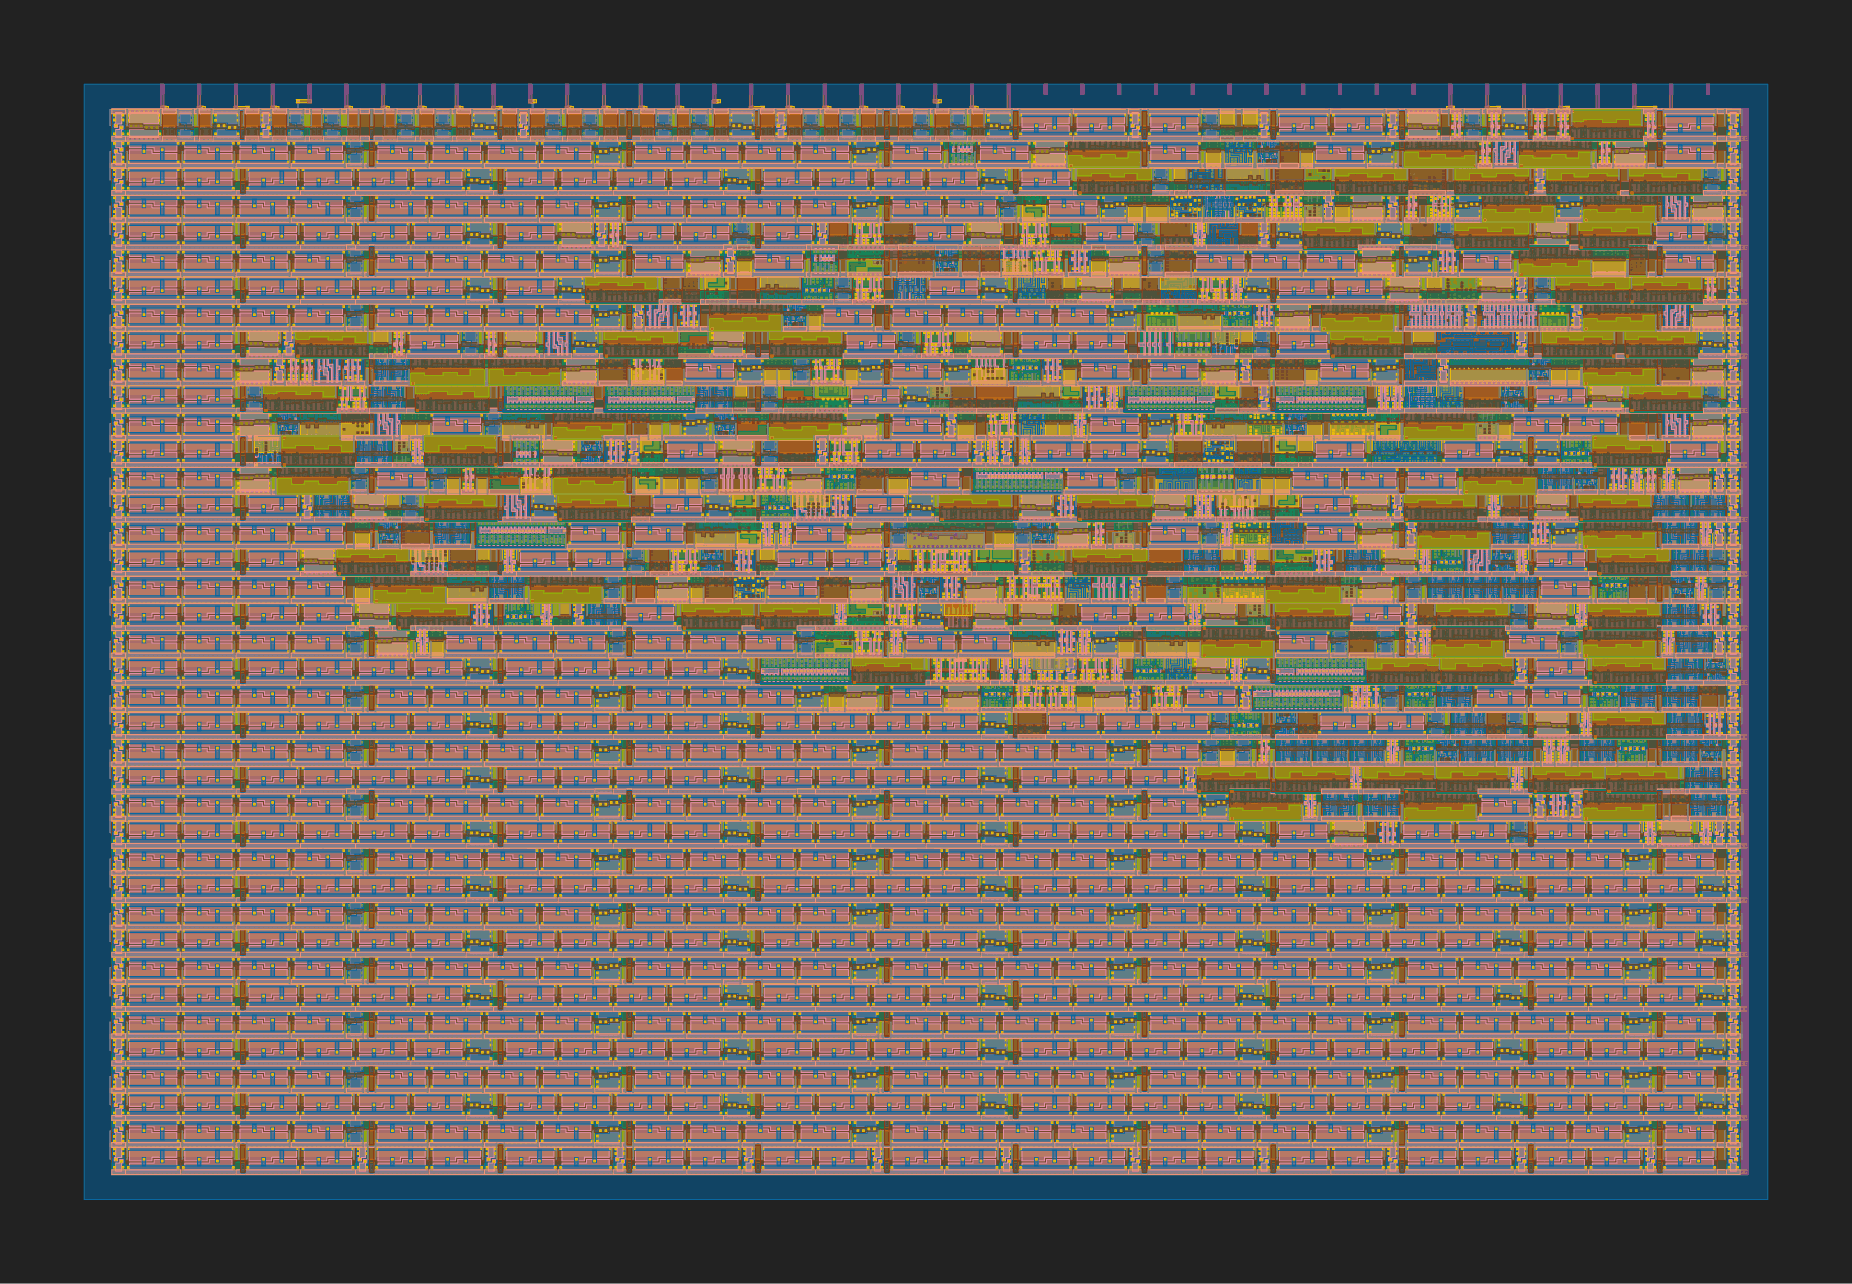
\includegraphics[width=\linewidth]{Pictures/Result_Pong_2D_View.png}
        \caption{View 2D}\label{fig:PWM_2D}
    \end{subfigure}
    \begin{subfigure}[b]{0.45\textwidth}
        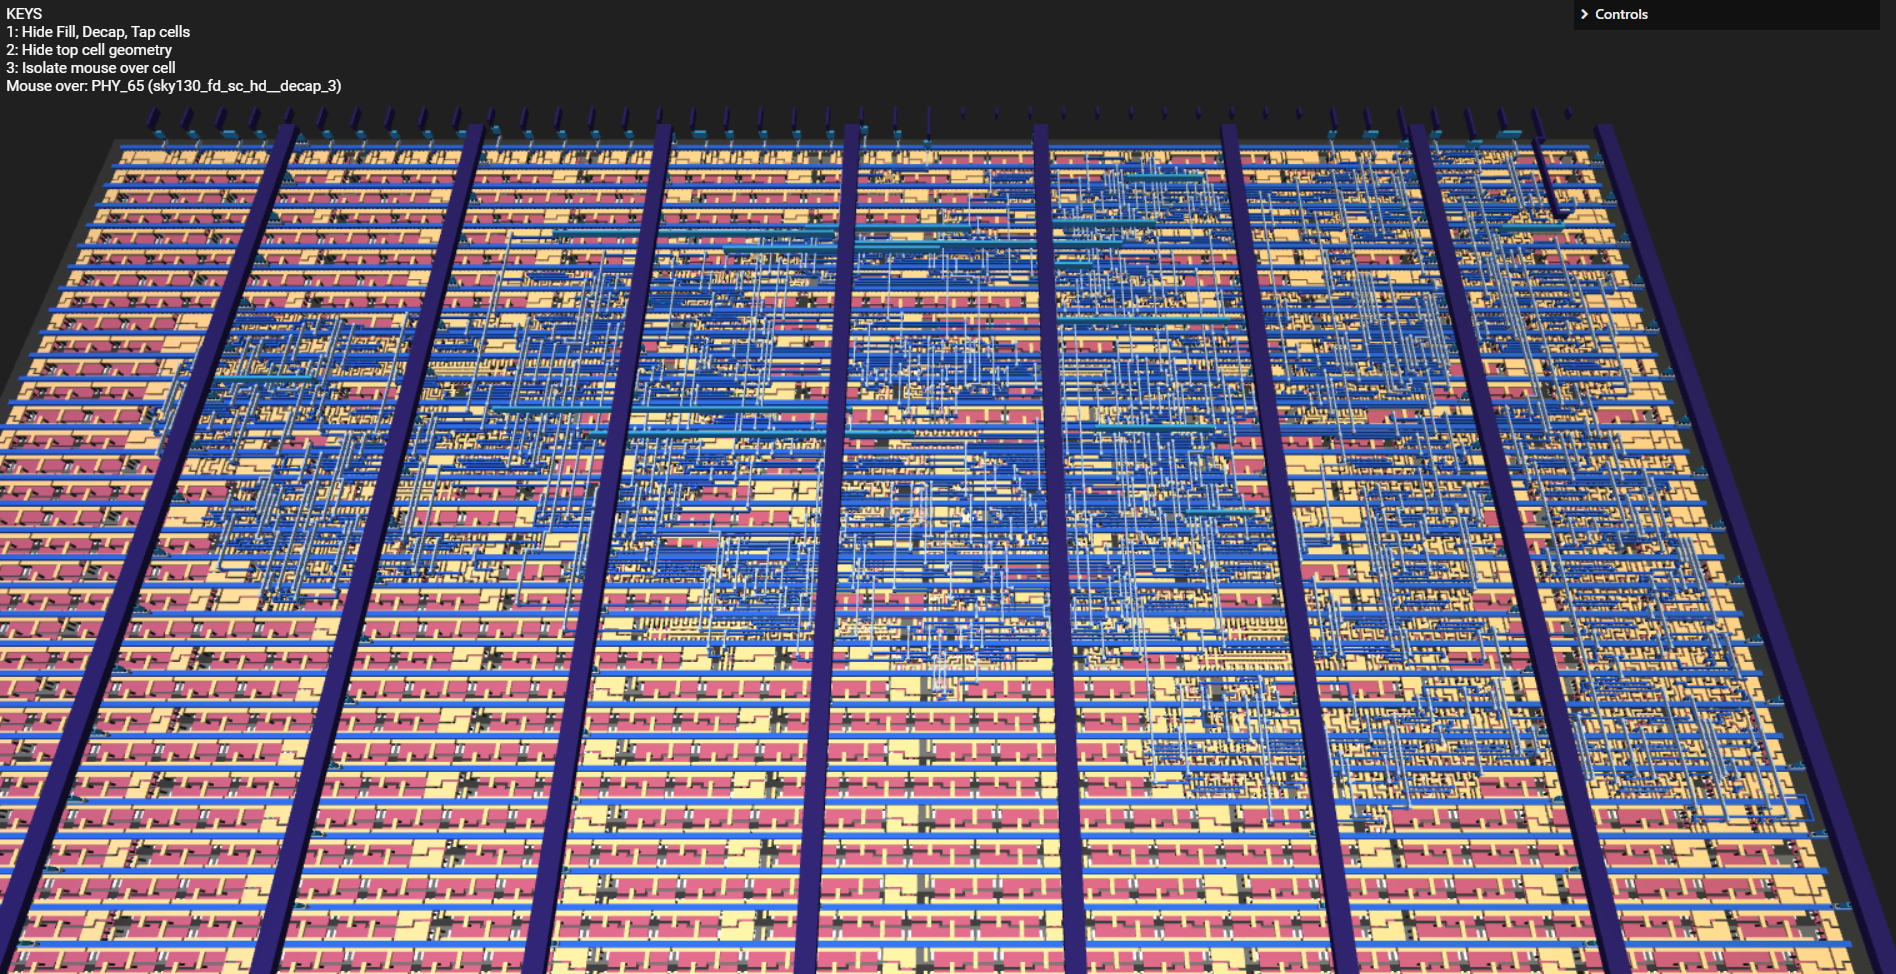
\includegraphics[width=\linewidth]{Pictures/Result_Pong_3D_View.png}
        \caption{View 3D}\label{fig:PWM_3D}
    \end{subfigure}
    \caption{The Pong game layout}\label{fig:PWM}
\end{figure}

subsection{Pulse Width Modulation Generator}

\begin{figure}[H]
    \centering
    \begin{subfigure}[b]{0.45\textwidth}
        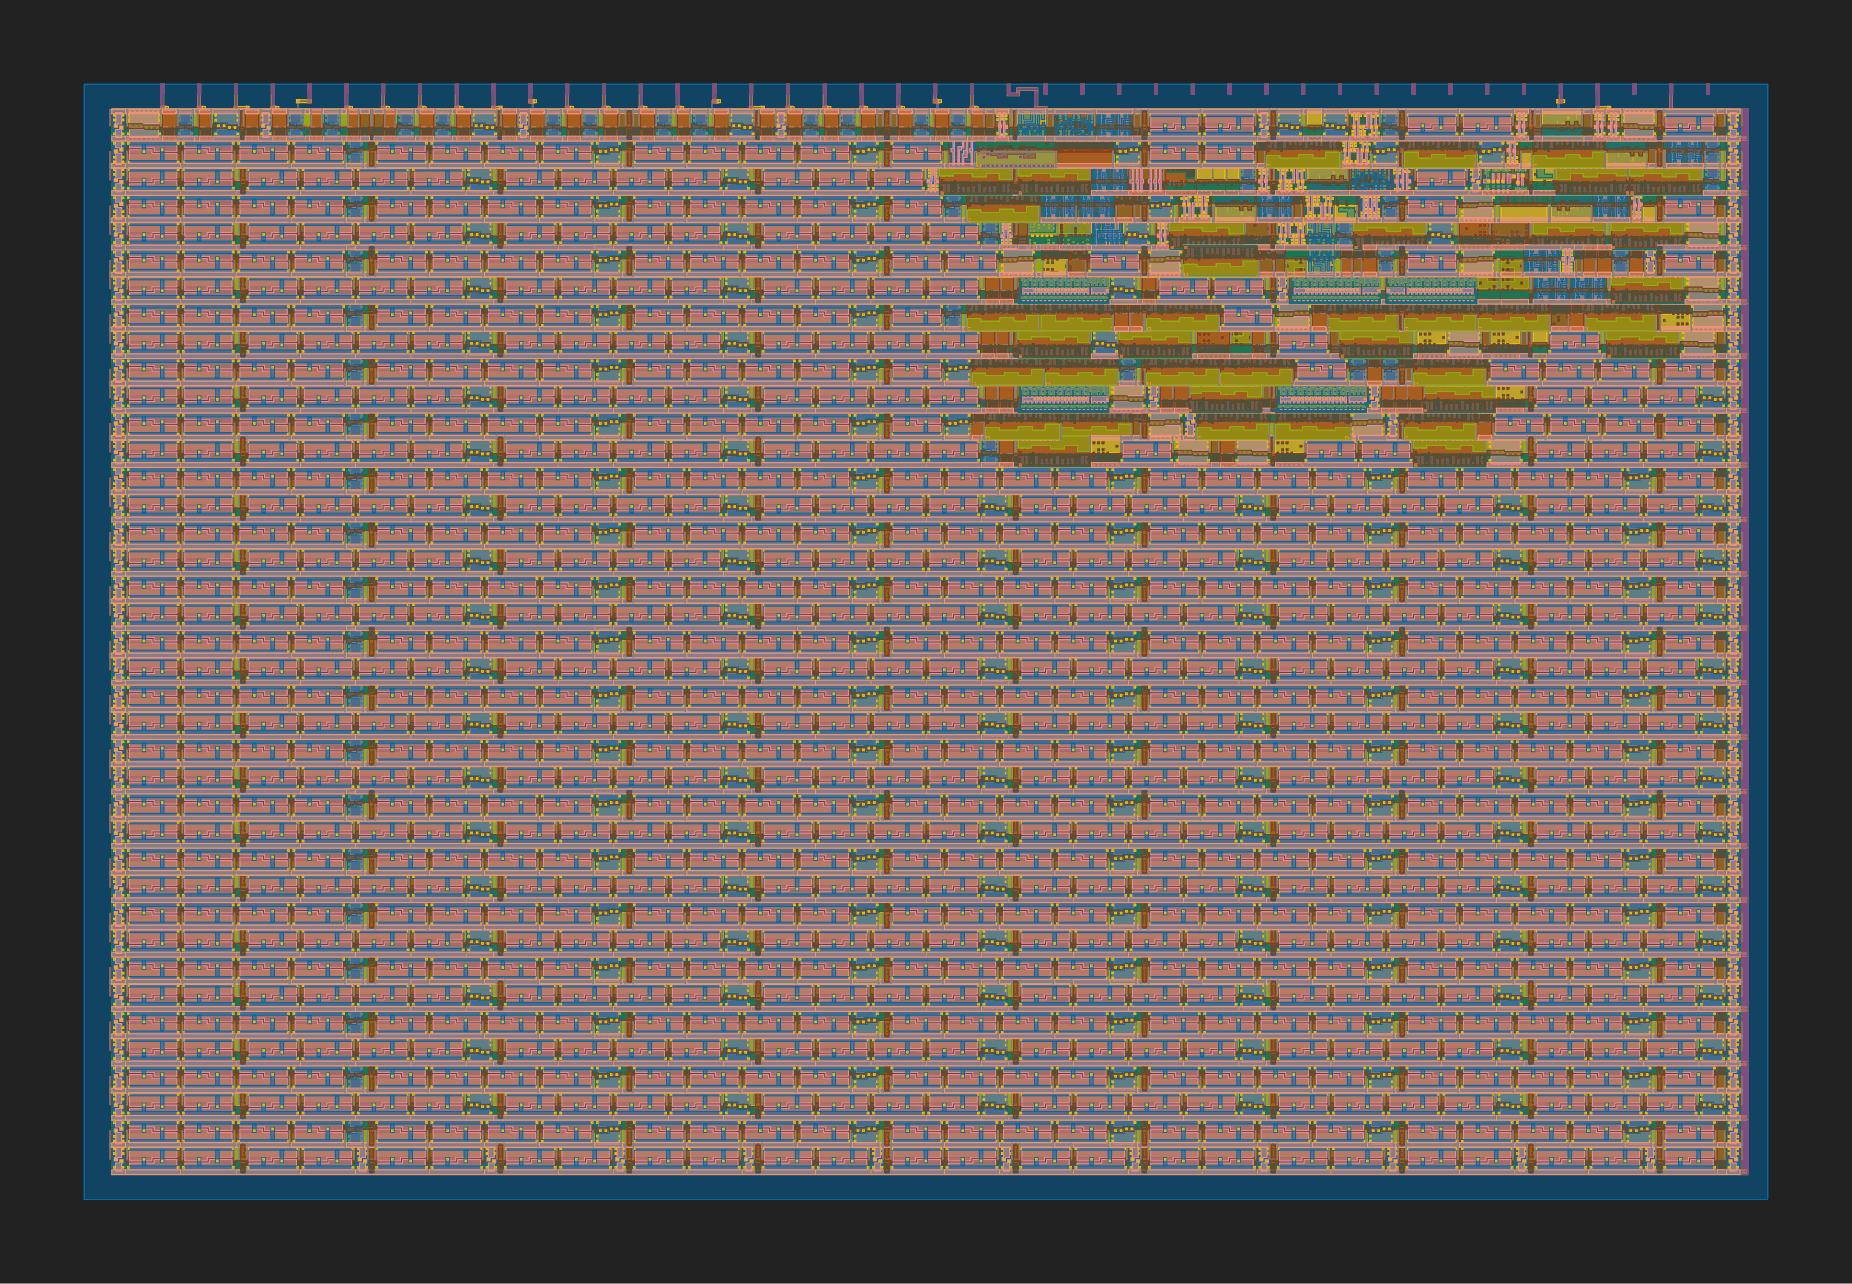
\includegraphics[width=\linewidth]{Pictures/Result_PWM_2D_View.png}
        \caption{View 2D}\label{fig:PWM_2D}
    \end{subfigure}
    \begin{subfigure}[b]{0.45\textwidth}
        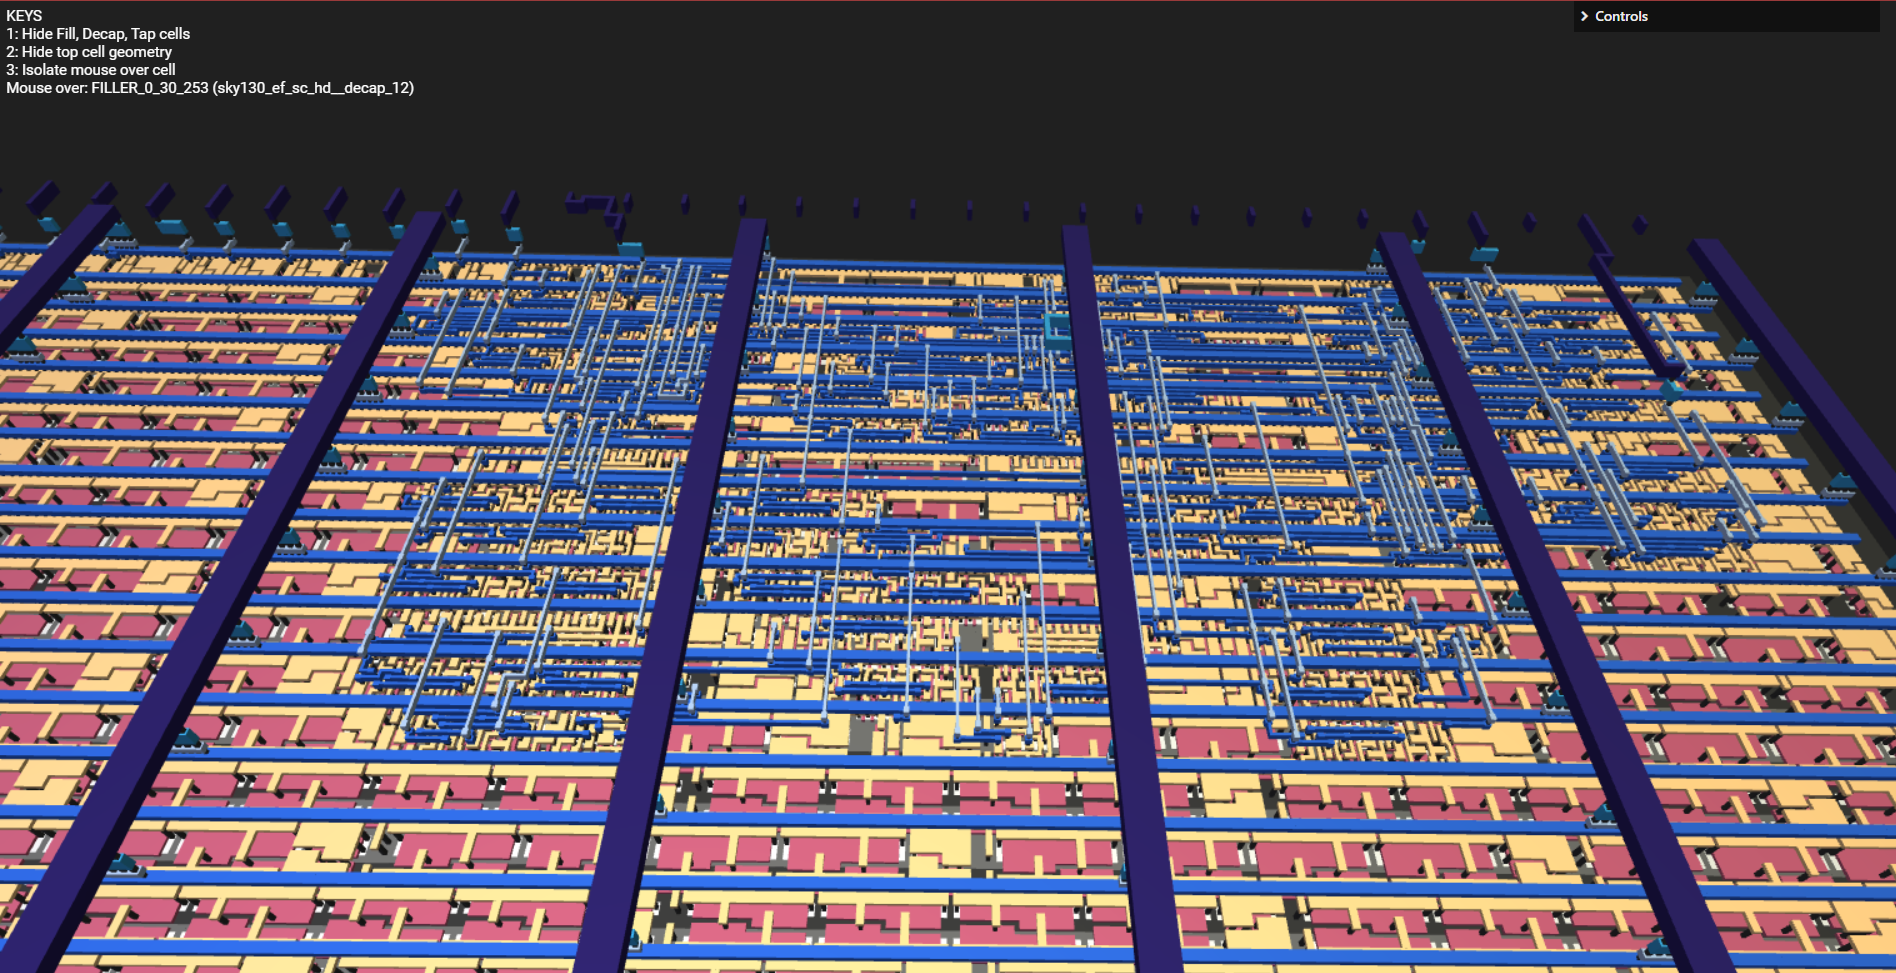
\includegraphics[width=\linewidth]{Pictures/Result_PWM_3D_View.png}
        \caption{View 3D}\label{fig:PWM_3D}
    \end{subfigure}
    \caption{Pulse Width Modulation generator layout}\label{fig:PWM}
\end{figure}


% Please add the following required packages to your document preamble:
% \usepackage{booktabs}
\begin{table}[H]
\centering
\begin{tabular}{@{}cc@{}}
\toprule
Circuit                                 & \begin{tabular}[c]{@{}c@{}}Porsentage utilize in \\ length of waver(\%)\end{tabular} \\ \midrule
Multi stage path for delay measurements & 0.63                                                                                 \\
ASCII Text Printer Circuit              & 17.87                                                                                \\
Implementation of the Pong game         & 28.82                                                                                \\
Pulse Width Modulation Generator        & 9.59                                                                                 \\ \bottomrule
\caption{Porsentage utilize in length of waver per circuit.}\label{tab:RoutingStats}
\end{tabular}
\end{table}